% Options for packages loaded elsewhere
\PassOptionsToPackage{unicode}{hyperref}
\PassOptionsToPackage{hyphens}{url}
%
\documentclass[
  ,
]{ctexart}
\usepackage{amsmath,amssymb}
\usepackage{lmodern}
\usepackage{iftex}
\ifPDFTeX
  \usepackage[T1]{fontenc}
  \usepackage[utf8]{inputenc}
  \usepackage{textcomp} % provide euro and other symbols
\else % if luatex or xetex
  \usepackage{unicode-math}
  \defaultfontfeatures{Scale=MatchLowercase}
  \defaultfontfeatures[\rmfamily]{Ligatures=TeX,Scale=1}
\fi
% Use upquote if available, for straight quotes in verbatim environments
\IfFileExists{upquote.sty}{\usepackage{upquote}}{}
\IfFileExists{microtype.sty}{% use microtype if available
  \usepackage[]{microtype}
  \UseMicrotypeSet[protrusion]{basicmath} % disable protrusion for tt fonts
}{}
\makeatletter
\@ifundefined{KOMAClassName}{% if non-KOMA class
  \IfFileExists{parskip.sty}{%
    \usepackage{parskip}
  }{% else
    \setlength{\parindent}{0pt}
    \setlength{\parskip}{6pt plus 2pt minus 1pt}}
}{% if KOMA class
  \KOMAoptions{parskip=half}}
\makeatother
\usepackage{xcolor}
\IfFileExists{xurl.sty}{\usepackage{xurl}}{} % add URL line breaks if available
\IfFileExists{bookmark.sty}{\usepackage{bookmark}}{\usepackage{hyperref}}
\hypersetup{
  pdftitle={面向非本领域读者的完整项目报告：可解释药物脂溶性预测平台},
  pdflang={zh-CN},
  hidelinks,
  pdfcreator={LaTeX via pandoc}}
\urlstyle{same} % disable monospaced font for URLs
\usepackage{longtable,booktabs,array}
\usepackage{calc} % for calculating minipage widths
% Correct order of tables after \paragraph or \subparagraph
\usepackage{etoolbox}
\makeatletter
\patchcmd\longtable{\par}{\if@noskipsec\mbox{}\fi\par}{}{}
\makeatother
% Allow footnotes in longtable head/foot
\IfFileExists{footnotehyper.sty}{\usepackage{footnotehyper}}{\usepackage{footnote}}
\makesavenoteenv{longtable}
\usepackage{graphicx}
\makeatletter
\def\maxwidth{\ifdim\Gin@nat@width>\linewidth\linewidth\else\Gin@nat@width\fi}
\def\maxheight{\ifdim\Gin@nat@height>\textheight\textheight\else\Gin@nat@height\fi}
\makeatother
% Scale images if necessary, so that they will not overflow the page
% margins by default, and it is still possible to overwrite the defaults
% using explicit options in \includegraphics[width, height, ...]{}
\setkeys{Gin}{width=\maxwidth,height=\maxheight,keepaspectratio}
% Set default figure placement to htbp
\makeatletter
\def\fps@figure{htbp}
\makeatother
\setlength{\emergencystretch}{3em} % prevent overfull lines
\providecommand{\tightlist}{%
  \setlength{\itemsep}{0pt}\setlength{\parskip}{0pt}}
\setcounter{secnumdepth}{-\maxdimen} % remove section numbering
\ifXeTeX
  % Load polyglossia as late as possible: uses bidi with RTL langages (e.g. Hebrew, Arabic)
  \usepackage{polyglossia}
  \setmainlanguage[]{}
\else
  \usepackage[main=]{babel}
% get rid of language-specific shorthands (see #6817):
\let\LanguageShortHands\languageshorthands
\def\languageshorthands#1{}
\fi
\ifLuaTeX
  \usepackage{selnolig}  % disable illegal ligatures
\fi

\title{面向非本领域读者的完整项目报告：可解释药物脂溶性预测平台}
\author{}
\date{}

\begin{document}
\maketitle

\hypertarget{ux9762ux5411ux975eux672cux9886ux57dfux8bfbux8005ux7684ux5b8cux6574ux9879ux76eeux62a5ux544aux53efux89e3ux91caux836fux7269ux8102ux6eb6ux6027ux9884ux6d4bux5e73ux53f0}{%
\section{面向非本领域读者的完整项目报告：可解释药物脂溶性预测平台}\label{ux9762ux5411ux975eux672cux9886ux57dfux8bfbux8005ux7684ux5b8cux6574ux9879ux76eeux62a5ux544aux53efux89e3ux91caux836fux7269ux8102ux6eb6ux6027ux9884ux6d4bux5e73ux53f0}}

\begin{quote}
版本：2026-03-15\\
项目目录：\texttt{/public/home/zhw/cptac/projects/experiment/qsar\_project}\\
适用对象：药学研究生复试、跨学科答辩、GitHub 项目介绍、Hugging Face
平台说明\\
读者假设：默认读者不同时具备药学、化学信息学和机器学习背景，因此本报告会先解释``为什么要做''，再解释``怎么做''，最后解释``结果意味着什么''。
\end{quote}

\begin{center}\rule{0.5\linewidth}{0.5pt}\end{center}

\hypertarget{ux4e00ux5148ux7528ux4e00ux53e5ux8bddux8bb2ux6e05ux695aux8fd9ux4e2aux9879ux76ee}{%
\subsection{一、先用一句话讲清楚这个项目}\label{ux4e00ux5148ux7528ux4e00ux53e5ux8bddux8bb2ux6e05ux695aux8fd9ux4e2aux9879ux76ee}}

这个项目做的事情是：

\textbf{根据一个分子的结构（SMILES），用真实公开数据训练得到的模型去预测它的脂溶性，并进一步用可解释性方法说明模型为什么这么判断，最后把结果做成可以直接访问的网页和
API。}

如果再口语一点，可以把它理解成：

\begin{quote}
这是一个``药物分子实验前预筛选助手''。
\end{quote}

你给它一个分子的结构，它先告诉你这个分子大概更偏亲水还是疏水，然后再告诉你：模型主要是根据哪些结构或理化特征做出这个判断的。这样，药化人员可以更有依据地决定：

\begin{itemize}
\tightlist
\item
  这个分子值不值得继续做实验；
\item
  如果想把它改得更亲水或更疏水，结构上可能往哪个方向修改更合理。
\end{itemize}

\begin{center}\rule{0.5\linewidth}{0.5pt}\end{center}

\hypertarget{ux4e8cux8fd9ux4e2aux9879ux76eeux4e3aux4ec0ux4e48ux91cdux8981}{%
\subsection{二、这个项目为什么重要}\label{ux4e8cux8fd9ux4e2aux9879ux76eeux4e3aux4ec0ux4e48ux91cdux8981}}

\hypertarget{ux836fux5b66ux80ccux666fux4e3aux4ec0ux4e48ux8981ux5173ux6ce8ux8102ux6eb6ux6027}{%
\subsubsection{2.1
药学背景：为什么要关注脂溶性}\label{ux836fux5b66ux80ccux666fux4e3aux4ec0ux4e48ux8981ux5173ux6ce8ux8102ux6eb6ux6027}}

脂溶性（lipophilicity，常见表征是 logD 或
logP）是药物研发中非常关键的性质。它会影响：

\begin{itemize}
\tightlist
\item
  \textbf{吸收（Absorption）}：分子能不能比较容易通过生物膜；
\item
  \textbf{分布（Distribution）}：进入体内后更容易停留在血液、水相环境，还是进入脂质丰富的组织；
\item
  \textbf{膜通透性（Membrane
  permeability）}：对口服药、脑靶向药等都很关键；
\item
  \textbf{成药性（Drug-likeness）}：太亲水或太疏水都可能带来问题。
\end{itemize}

可以粗略理解为：

\begin{itemize}
\tightlist
\item
  \textbf{脂溶性太低}：分子可能不容易穿膜，吸收差；
\item
  \textbf{脂溶性太高}：分子虽然更容易穿膜，但可能溶解性差、非特异性结合增多、体内暴露不可控。
\end{itemize}

所以在药物设计里，脂溶性经常不是``越高越好''或``越低越好''，而是\textbf{要平衡}。

\hypertarget{ux73b0ux5b9eux75dbux70b9ux5b9eux9a8cux53efux9760ux4f46ux4ee3ux4ef7ux9ad8}{%
\subsubsection{2.2
现实痛点：实验可靠，但代价高}\label{ux73b0ux5b9eux75dbux70b9ux5b9eux9a8cux53efux9760ux4f46ux4ee3ux4ef7ux9ad8}}

当然，最可靠的办法始终是做实验测量。但实验存在几个现实问题：

\begin{itemize}
\tightlist
\item
  成本高；
\item
  周期长；
\item
  不能对大量候选分子都优先做完实验再决策。
\end{itemize}

因此，一个很自然的问题是：

\begin{quote}
能不能在实验之前，先用计算方法做一次``预筛选''？
\end{quote}

这就是本项目的切入点。

\begin{center}\rule{0.5\linewidth}{0.5pt}\end{center}

\hypertarget{ux4e09ux8fd9ux4e2aux9879ux76eeux5230ux5e95ux89e3ux51b3ux4e86ux4ec0ux4e48ux95eeux9898}{%
\subsection{三、这个项目到底解决了什么问题}\label{ux4e09ux8fd9ux4e2aux9879ux76eeux5230ux5e95ux89e3ux51b3ux4e86ux4ec0ux4e48ux95eeux9898}}

项目的目标不是做一个``花哨的模型''，而是解决一个\textbf{真实的研发决策问题}：

\begin{quote}
对一个新分子，在还没做实验之前，我们能不能基于结构大致判断它的脂溶性，并给出可解释的结构层面提示？
\end{quote}

因此，这个项目有三个层次的目标：

\begin{enumerate}
\def\labelenumi{\arabic{enumi}.}
\tightlist
\item
  \textbf{预测层}：模型能不能把脂溶性预测得比较准；
\item
  \textbf{验证层}：模型是不是只在随机划分里看起来很厉害，还是在更严格设定下依然稳；
\item
  \textbf{解释层}：模型能不能告诉我们``为什么这么判断''，而不是只给一个数。
\end{enumerate}

再往前走一步，我们还把它做成了一个小型平台，所以还有第四层目标：

\begin{enumerate}
\def\labelenumi{\arabic{enumi}.}
\setcounter{enumi}{3}
\tightlist
\item
  \textbf{平台层}：别人能不能不看代码、直接打开网页体验这个项目。
\end{enumerate}

\begin{center}\rule{0.5\linewidth}{0.5pt}\end{center}

\hypertarget{ux56dbux9879ux76eeux7684ux5b8cux6574ux5de5ux4f5cux6d41ux4eceux5934ux5230ux5c3e}{%
\subsection{四、项目的完整工作流（从头到尾）}\label{ux56dbux9879ux76eeux7684ux5b8cux6574ux5de5ux4f5cux6d41ux4eceux5934ux5230ux5c3e}}

这个项目可以分成 9 个步骤：

\begin{enumerate}
\def\labelenumi{\arabic{enumi}.}
\tightlist
\item
  明确研究问题\\
\item
  获取真实公开数据\\
\item
  清洗与标准化分子结构\\
\item
  构建多种分子特征\\
\item
  训练基线模型与增强模型\\
\item
  比较模型性能\\
\item
  做更严格的 scaffold 验证\\
\item
  做 SHAP 可解释性分析\\
\item
  做成网页平台与 API
\end{enumerate}

下面逐步解释。

\begin{center}\rule{0.5\linewidth}{0.5pt}\end{center}

\hypertarget{ux4e94ux6570ux636eux4eceux54eaux91ccux6765ux4e3aux4ec0ux4e48ux53efux4fe1}{%
\subsection{五、数据从哪里来，为什么可信}\label{ux4e94ux6570ux636eux4eceux54eaux91ccux6765ux4e3aux4ec0ux4e48ux53efux4fe1}}

\hypertarget{ux6570ux636eux6765ux6e90}{%
\subsubsection{5.1 数据来源}\label{ux6570ux636eux6765ux6e90}}

本项目使用的是公开 \texttt{Lipophilicity} 数据集，来自 MoleculeNet /
DeepChem 体系，对应真实药物样分子的实验脂溶性记录。

项目中已经整理的数据概况：

\begin{itemize}
\tightlist
\item
  数据集规模：\texttt{4200} 个分子
\item
  目标变量：实验脂溶性（logD）
\item
  数据来源特征：包含 \texttt{ChEMBL} 编号
\item
  项目内摘要文件：\texttt{results/dataset\_summary.json}
\end{itemize}

\hypertarget{ux4e3aux4ec0ux4e48ux8fd9ux70b9ux91cdux8981}{%
\subsubsection{5.2
为什么这点重要}\label{ux4e3aux4ec0ux4e48ux8fd9ux70b9ux91cdux8981}}

这意味着：

\begin{itemize}
\tightlist
\item
  不是自己随手构造的模拟数据；
\item
  不是为了``做高分''专门拼凑的数据；
\item
  数据背后有公开数据库来源，可以追溯。
\end{itemize}

对于药学复试来说，这一点非常关键。因为老师往往不只关心你``会不会调模型''，还关心你：

\begin{itemize}
\tightlist
\item
  会不会处理真实科研数据；
\item
  知不知道公开数据库的重要性；
\item
  有没有可复现意识。
\end{itemize}

\hypertarget{ux6570ux636eux6e05ux6d17ux505aux4e86ux4ec0ux4e48}{%
\subsubsection{5.3
数据清洗做了什么}\label{ux6570ux636eux6e05ux6d17ux505aux4e86ux4ec0ux4e48}}

项目先对原始数据做了这些处理：

\begin{itemize}
\tightlist
\item
  校验 \texttt{SMILES} 是否能被 RDKit 正确解析；
\item
  统一成标准化结构表示；
\item
  去掉无效或重复结构；
\item
  保留可用于建模的真实标签。
\end{itemize}

可以理解为：

\begin{quote}
在开始训练模型之前，先把``分子结构数据''变成干净、统一、可计算的输入。
\end{quote}

\begin{center}\rule{0.5\linewidth}{0.5pt}\end{center}

\hypertarget{ux516dux600eux4e48ux628aux5206ux5b50ux53d8ux6210ux673aux5668ux80fdux7406ux89e3ux7684ux6570ux5b57}{%
\subsection{六、怎么把分子变成机器能理解的数字}\label{ux516dux600eux4e48ux628aux5206ux5b50ux53d8ux6210ux673aux5668ux80fdux7406ux89e3ux7684ux6570ux5b57}}

一个分子的 \texttt{SMILES} 是字符串，不能直接喂给机器学习模型。\\
所以我们必须把分子结构转成数字特征。这个过程叫 \textbf{特征工程}。

本项目使用了三类特征。

\hypertarget{ux57faux7840ux7406ux5316ux63cfux8ff0ux7b26}{%
\subsubsection{6.1
基础理化描述符}\label{ux57faux7840ux7406ux5316ux63cfux8ff0ux7b26}}

这类特征偏``药学常识''，代表分子的整体性质，例如：

\begin{itemize}
\tightlist
\item
  \texttt{MolWt}：分子量
\item
  \texttt{MolLogP}：疏水性/脂溶性相关指标
\item
  \texttt{TPSA}：拓扑极性表面积
\item
  \texttt{HBD/HBA}：氢键供体/受体数
\item
  \texttt{RingCount}：环数
\item
  \texttt{QED}：类药性评分
\end{itemize}

这类特征好处是：

\begin{itemize}
\tightlist
\item
  容易解释；
\item
  和药学语言直接对应；
\item
  很适合答辩时讲清楚模型在学什么。
\end{itemize}

\hypertarget{rdkit-ux5168ux91cf-2d-ux63cfux8ff0ux7b26}{%
\subsubsection{6.2 RDKit 全量 2D
描述符}\label{rdkit-ux5168ux91cf-2d-ux63cfux8ff0ux7b26}}

除了基础描述符之外，项目进一步计算了更全面的 2D
描述符，然后在训练集内做筛选：

\begin{itemize}
\tightlist
\item
  去掉缺失列；
\item
  去掉零方差列；
\item
  去掉高度相关列。
\end{itemize}

最后保留了 \textbf{173 个有效描述符}。

这一步的意义是：

\begin{itemize}
\tightlist
\item
  让模型看到更多结构相关信息；
\item
  但又避免无效特征和冗余特征拖累模型。
\end{itemize}

\hypertarget{ux5206ux5b50ux6307ux7eb9morgan-maccs}{%
\subsubsection{6.3 分子指纹：Morgan +
MACCS}\label{ux5206ux5b50ux6307ux7eb9morgan-maccs}}

这类特征更像``结构片段编码''。

\begin{itemize}
\tightlist
\item
  \textbf{Morgan Fingerprint}：描述分子局部原子环境和子结构模式；
\item
  \textbf{MACCS Keys}：描述常见结构键和化学片段是否存在。
\end{itemize}

可以把它们粗略理解成：

\begin{quote}
描述符更像``分子的整体体检报告''，\\
指纹更像``分子有哪些局部结构片段的编码表''。
\end{quote}

\hypertarget{ux4e3aux4ec0ux4e48ux8981ux591aux79cdux7279ux5f81ux4e00ux8d77ux7528}{%
\subsubsection{6.4
为什么要多种特征一起用}\label{ux4e3aux4ec0ux4e48ux8981ux591aux79cdux7279ux5f81ux4e00ux8d77ux7528}}

因为脂溶性这个性质不是由单一因素决定的。

它既和：

\begin{itemize}
\tightlist
\item
  分子整体大小、极性、氢键能力
\end{itemize}

有关，也和：

\begin{itemize}
\tightlist
\item
  某些具体结构片段、官能团、骨架模式
\end{itemize}

有关。

所以本项目选择：

\begin{quote}
\textbf{基础描述符 + 扩展描述符 + 结构指纹}
\end{quote}

来共同表达分子。

\begin{center}\rule{0.5\linewidth}{0.5pt}\end{center}

\hypertarget{ux4e03ux6a21ux578bux662fux600eux4e48ux4e00ux6b65ux6b65ux5347ux7ea7ux7684}{%
\subsection{七、模型是怎么一步步升级的}\label{ux4e03ux6a21ux578bux662fux600eux4e48ux4e00ux6b65ux6b65ux5347ux7ea7ux7684}}

\hypertarget{ux5148ux505aux57faux7ebfux6a21ux578b}{%
\subsubsection{7.1
先做基线模型}\label{ux5148ux505aux57faux7ebfux6a21ux578b}}

我们没有一上来就堆复杂方法，而是先做了几类基线模型：

\begin{itemize}
\tightlist
\item
  随机森林（Random Forest）
\item
  支持向量回归（SVR）
\item
  基线版 XGBoost
\end{itemize}

这样做的好处是：

\begin{itemize}
\tightlist
\item
  先知道一个合理起点；
\item
  后续每次升级都能比较``到底有没有真正进步''。
\end{itemize}

\hypertarget{ux505aux589eux5f3aux6a21ux578b}{%
\subsubsection{7.2 做增强模型}\label{ux505aux589eux5f3aux6a21ux578b}}

在增强版里，项目引入了：

\begin{itemize}
\tightlist
\item
  增强特征输入（描述符 + Morgan + MACCS）
\item
  XGBoost（增强版）
\item
  CatBoost
\item
  PyTorch MLP
\item
  加权集成（Weighted Ensemble）
\end{itemize}

这里的思路不是``哪个模型最炫就用哪个''，而是：

\begin{itemize}
\tightlist
\item
  树模型（XGBoost / CatBoost）对结构化特征很强；
\item
  MLP 可以学习高维连续特征的复杂组合；
\item
  三者的错误模式并不完全一样；
\item
  所以做集成往往能更稳。
\end{itemize}

\hypertarget{ux4e3aux4ec0ux4e48ux96c6ux6210ux6a21ux578bux662fux6700ux7ec8ux6700ux4f18ux89e3}{%
\subsubsection{7.3
为什么集成模型是最终最优解}\label{ux4e3aux4ec0ux4e48ux96c6ux6210ux6a21ux578bux662fux6700ux7ec8ux6700ux4f18ux89e3}}

最终最佳模型是：

\begin{itemize}
\tightlist
\item
  \texttt{Weighted\_Ensemble\_rich}
\end{itemize}

它本质上不是重新训练了一个更复杂的``大一统模型''，而是：

\begin{itemize}
\tightlist
\item
  把 XGBoost、CatBoost、MLP 的输出按验证集上优化得到的权重做组合。
\end{itemize}

也就是说：

\begin{quote}
我们不是盲目追求``单个模型必须赢''，而是利用不同模型之间的互补性。
\end{quote}

这是一种很典型、也很成熟的工程与科研思路。

\begin{center}\rule{0.5\linewidth}{0.5pt}\end{center}

\hypertarget{ux516bux6a21ux578bux5230ux5e95ux8868ux73b0ux600eux4e48ux6837}{%
\subsection{八、模型到底表现怎么样}\label{ux516bux6a21ux578bux5230ux5e95ux8868ux73b0ux600eux4e48ux6837}}

\hypertarget{ux666eux901aux6d4bux8bd5ux96c6ux7ed3ux679c}{%
\subsubsection{8.1
普通测试集结果}\label{ux666eux901aux6d4bux8bd5ux96c6ux7ed3ux679c}}

增强版最终结果如下（来自 \texttt{results/final\_results\_v2.md}）：

\begin{longtable}[]{@{}lrrr@{}}
\toprule
模型 & R² & RMSE & MAE \\
\midrule
\endhead
Weighted\_Ensemble\_rich & 0.7232 & 0.6346 & 0.4517 \\
XGB\_rich\_desc\_fp\_maccs & 0.7043 & 0.6559 & 0.4810 \\
CatBoost\_rich\_desc\_fp\_maccs & 0.6973 & 0.6637 & 0.4862 \\
PyTorch\_MLP\_rich\_desc\_fp\_maccs & 0.6967 & 0.6643 & 0.4634 \\
XGB\_baseline\_desc\_fp & 0.6835 & 0.6787 & 0.5075 \\
\bottomrule
\end{longtable}

\hypertarget{ux8fd9ux4e9bux6570ux5b57ux600eux4e48ux7406ux89e3}{%
\subsubsection{8.2
这些数字怎么理解}\label{ux8fd9ux4e9bux6570ux5b57ux600eux4e48ux7406ux89e3}}

\begin{itemize}
\tightlist
\item
  \textbf{R² 越高越好}：表示模型对真实变化的解释能力更强；
\item
  \textbf{RMSE 越低越好}：表示预测误差更小；
\item
  \textbf{MAE 越低越好}：表示平均绝对偏差更小。
\end{itemize}

从结果上看：

\begin{itemize}
\tightlist
\item
  增强版模型整体优于基线；
\item
  集成模型最好；
\item
  深度学习模型单独也很强，但最终集成更稳。
\end{itemize}

\hypertarget{ux76f8ux6bd4ux4e0aux4e00ux7248ux63d0ux5347ux4e86ux4ec0ux4e48}{%
\subsubsection{8.3
相比上一版提升了什么}\label{ux76f8ux6bd4ux4e0aux4e00ux7248ux63d0ux5347ux4e86ux4ec0ux4e48}}

上一版最佳是：

\begin{itemize}
\tightlist
\item
  \texttt{XGB\_desc\_fp}
\item
  Test \texttt{R²\ =\ 0.6835}
\item
  Test \texttt{RMSE\ =\ 0.6787}
\end{itemize}

增强版最佳是：

\begin{itemize}
\tightlist
\item
  \texttt{Weighted\_Ensemble\_rich}
\item
  Test \texttt{R²\ =\ 0.7232}
\item
  Test \texttt{RMSE\ =\ 0.6346}
\end{itemize}

也就是：

\begin{itemize}
\tightlist
\item
  \texttt{R²} 提升了 \texttt{0.0397}
\item
  \texttt{RMSE} 降低了 \texttt{0.0440}
\end{itemize}

这说明增强并不是``做了很多事但没效果''，而是带来了明确收益。

\begin{center}\rule{0.5\linewidth}{0.5pt}\end{center}

\hypertarget{ux4e5dux4e3aux4ec0ux4e48ux8fd8ux8981ux505aux66f4ux4e25ux683cux7684ux9a8cux8bc1}{%
\subsection{九、为什么还要做更严格的验证}\label{ux4e5dux4e3aux4ec0ux4e48ux8fd8ux8981ux505aux66f4ux4e25ux683cux7684ux9a8cux8bc1}}

如果只做普通随机划分，老师可能会问：

\begin{quote}
这些分子是不是在训练集和测试集里其实很像，所以模型看起来很厉害？
\end{quote}

这个问题非常关键。因为在真实药物研发里，模型常常面对的是：

\begin{itemize}
\tightlist
\item
  一个\textbf{新骨架（new scaffold）}的分子，
\item
  而不是和训练集高度相似的分子。
\end{itemize}

\hypertarget{ux4ec0ux4e48ux662f-scaffold-split}{%
\subsubsection{9.1 什么是 scaffold
split}\label{ux4ec0ux4e48ux662f-scaffold-split}}

scaffold 可以理解为分子的``骨架框架''。\\
如果训练集和测试集共享大量相似骨架，那么模型在测试集上的表现可能会偏乐观。

所以项目进一步加入了：

\begin{itemize}
\tightlist
\item
  \textbf{5 次 repeated scaffold split}
\end{itemize}

也就是说：

\begin{itemize}
\tightlist
\item
  让训练集和测试集尽量在骨架层面分开；
\item
  重复多次，计算平均值和标准差；
\item
  看模型是否稳定，而不是只看一次运气。
\end{itemize}

\hypertarget{ux4e25ux683cux9a8cux8bc1ux7ed3ux679c}{%
\subsubsection{9.2
严格验证结果}\label{ux4e25ux683cux9a8cux8bc1ux7ed3ux679c}}

来自 \texttt{results/scaffold\_validation\_results.md}：

\begin{longtable}[]{@{}lrrr@{}}
\toprule
模型 & R² mean ± std & RMSE mean ± std & MAE mean ± std \\
\midrule
\endhead
Weighted\_Ensemble\_scaffold & 0.7138 ± 0.0215 & 0.6489 ± 0.0296 &
0.4962 ± 0.0226 \\
PyTorch\_MLP\_rich\_scaffold & 0.6945 ± 0.0261 & 0.6698 ± 0.0200 &
0.5111 ± 0.0187 \\
XGB\_rich\_scaffold & 0.6847 ± 0.0234 & 0.6811 ± 0.0347 & 0.5241 ±
0.0252 \\
CatBoost\_rich\_scaffold & 0.6750 ± 0.0234 & 0.6914 ± 0.0295 & 0.5313 ±
0.0201 \\
XGB\_baseline\_scaffold & 0.6472 ± 0.0311 & 0.7200 ± 0.0299 & 0.5519 ±
0.0234 \\
\bottomrule
\end{longtable}

\hypertarget{ux4e3aux4ec0ux4e48ux8fd9ux7ec4ux7ed3ux679cux5f88ux91cdux8981}{%
\subsubsection{9.3
为什么这组结果很重要}\label{ux4e3aux4ec0ux4e48ux8fd9ux7ec4ux7ed3ux679cux5f88ux91cdux8981}}

这组结果通常会比随机划分更低，这是\textbf{正常的}。因为验证变严格了。

真正重要的是：

\begin{itemize}
\tightlist
\item
  增强版在严格 scaffold 设定下依然明显优于基线；
\item
  集成模型依然是最优；
\item
  标准差不大，说明重复实验比较稳定。
\end{itemize}

这会让老师觉得你不是只会``做一个漂亮分数''，而是知道：

\begin{quote}
\textbf{科研里要证明模型真的能泛化。}
\end{quote}

\begin{center}\rule{0.5\linewidth}{0.5pt}\end{center}

\hypertarget{ux5341shap-ux548c-xai-ux5230ux5e95ux8bc1ux660eux4e86ux4ec0ux4e48}{%
\subsection{十、SHAP 和 XAI
到底证明了什么}\label{ux5341shap-ux548c-xai-ux5230ux5e95ux8bc1ux660eux4e86ux4ec0ux4e48}}

很多模型预测项目只停留在：

\begin{itemize}
\tightlist
\item
  输入分子
\item
  输出一个数字
\end{itemize}

但这在答辩里很容易被追问：

\begin{itemize}
\tightlist
\item
  模型为什么这么判断？
\item
  你怎么证明它学到的是有意义的东西？
\item
  这个结果对药化修改有什么指导价值？
\end{itemize}

所以项目加了 \textbf{SHAP（SHapley Additive
exPlanations）}，这就是一类典型的 \textbf{XAI（可解释人工智能）} 方法。

\hypertarget{shap-ux7684ux4e24ux4e2aux5c42ux9762}{%
\subsubsection{10.1 SHAP
的两个层面}\label{shap-ux7684ux4e24ux4e2aux5c42ux9762}}

\hypertarget{ux5168ux5c40ux89e3ux91ca}{%
\paragraph{全局解释}\label{ux5168ux5c40ux89e3ux91ca}}

说明整个模型最重视哪些特征。

项目中排名靠前的特征包括：

\begin{itemize}
\tightlist
\item
  \texttt{MolLogP}
\item
  \texttt{fr\_COO}
\item
  \texttt{VSA\_EState5}
\item
  \texttt{MACCS\_104}
\item
  \texttt{SMR\_VSA10}
\end{itemize}

这很有意义，因为：

\begin{itemize}
\tightlist
\item
  \texttt{MolLogP} 和脂溶性本身高度相关；
\item
  酸性基团、极性表面积等也会影响分子在水相/脂相中的分配行为；
\item
  说明模型并不是在抓毫无意义的噪声。
\end{itemize}

\hypertarget{ux5c40ux90e8ux89e3ux91ca}{%
\paragraph{局部解释}\label{ux5c40ux90e8ux89e3ux91ca}}

说明对\textbf{某一个具体分子}，哪些特征在把预测值往上推，哪些在往下拉。

项目还专门挑了 3 个案例：

\begin{itemize}
\tightlist
\item
  \texttt{HighPrediction}
\item
  \texttt{LowPrediction}
\item
  \texttt{LargeError}
\end{itemize}

这样就能回答：

\begin{quote}
为什么这个分子会被预测成高脂溶性？\\
为什么另一个分子会被预测成低脂溶性？\\
为什么有的分子模型会判断失误？
\end{quote}

\hypertarget{shap-ux5bf9ux7b54ux8fa9ux7684ux4ef7ux503c}{%
\subsubsection{10.2 SHAP
对答辩的价值}\label{shap-ux5bf9ux7b54ux8fa9ux7684ux4ef7ux503c}}

SHAP 不能证明因果，但它能证明：

\begin{itemize}
\tightlist
\item
  模型判断有迹可循；
\item
  重要特征与药学常识相符；
\item
  对单个分子可以给出``结构方向上的解释提示''。
\end{itemize}

你可以把它理解成：

\begin{quote}
SHAP 让这个项目从``黑盒预测器''升级成``可解释的药化辅助工具''。
\end{quote}

\begin{center}\rule{0.5\linewidth}{0.5pt}\end{center}

\hypertarget{ux5341ux4e00ux8fd9ux4e2aux9879ux76eeux505aux6210ux5e73ux53f0ux610fux5473ux7740ux4ec0ux4e48}{%
\subsection{十一、这个项目做成平台意味着什么}\label{ux5341ux4e00ux8fd9ux4e2aux9879ux76eeux505aux6210ux5e73ux53f0ux610fux5473ux7740ux4ec0ux4e48}}

很多课程项目只到``代码能跑''和``图画出来''为止。\\
但这个项目进一步做成了：

\begin{itemize}
\tightlist
\item
  网页前端
\item
  JSON API
\item
  Hugging Face Space 可部署演示平台
\end{itemize}

\hypertarget{ux5e73ux53f0ux53efux4ee5ux5e72ux4ec0ux4e48}{%
\subsubsection{11.1
平台可以干什么}\label{ux5e73ux53f0ux53efux4ee5ux5e72ux4ec0ux4e48}}

用户可以：

\begin{itemize}
\tightlist
\item
  输入一个新的 \texttt{SMILES}
\item
  得到脂溶性预测值
\item
  看到结构图
\item
  看到正向和负向 SHAP 特征
\item
  查看项目核心结果图
\item
  查看严格验证结果
\item
  通过 API 调用预测接口
\end{itemize}

\hypertarget{ux8fd9ux4e3aux4ec0ux4e48ux91cdux8981}{%
\subsubsection{11.2
这为什么重要}\label{ux8fd9ux4e3aux4ec0ux4e48ux91cdux8981}}

因为这说明你不仅会：

\begin{itemize}
\tightlist
\item
  训练模型
\item
  解释模型
\end{itemize}

你还会：

\begin{itemize}
\tightlist
\item
  把模型包装成别人可以直接使用的工具
\item
  考虑部署与调用方式
\item
  考虑作品展示和工程落地
\end{itemize}

对计算机老师来说，这体现工程能力。\\
对药学老师来说，这意味着项目更接近``真的能用''的科研工具。

\begin{center}\rule{0.5\linewidth}{0.5pt}\end{center}

\hypertarget{ux5341ux4e8cgemini-ux5728ux8fd9ux4e2aux9879ux76eeux91ccux626eux6f14ux4ec0ux4e48ux89d2ux8272}{%
\subsection{十二、Gemini
在这个项目里扮演什么角色}\label{ux5341ux4e8cgemini-ux5728ux8fd9ux4e2aux9879ux76eeux91ccux626eux6f14ux4ec0ux4e48ux89d2ux8272}}

Gemini
不是这个项目的\textbf{核心预测模型}，而是一个\textbf{辅助解释层}。

它的作用不是替代现有模型，而是把已有结果翻译得更适合人读。

\hypertarget{ux6838ux5fc3ux6a21ux578bux548c-gemini-ux7684ux5206ux5de5}{%
\subsubsection{12.1 核心模型和 Gemini
的分工}\label{ux6838ux5fc3ux6a21ux578bux548c-gemini-ux7684ux5206ux5de5}}

\begin{itemize}
\tightlist
\item
  \textbf{核心模型}负责：

  \begin{itemize}
  \tightlist
  \item
    真实预测脂溶性
  \item
    产生数值结果
  \item
    产生 SHAP 特征贡献
  \end{itemize}
\item
  \textbf{Gemini}负责：

  \begin{itemize}
  \tightlist
  \item
    把这些结果转换成更自然的中文说明
  \item
    生成药化优化建议
  \item
    输出适合答辩、展示或报告的语言版本
  \end{itemize}
\end{itemize}

\hypertarget{ux4e3aux4ec0ux4e48ux8fd9ux6837ux8bbeux8ba1ux662fux5408ux7406ux7684}{%
\subsubsection{12.2
为什么这样设计是合理的}\label{ux4e3aux4ec0ux4e48ux8fd9ux6837ux8bbeux8ba1ux662fux5408ux7406ux7684}}

因为如果让 Gemini 直接``猜脂溶性''，那就失去了严格建模和可验证性。\\
而现在的做法是：

\begin{quote}
先用真实训练得到的模型做预测，\\
再用 Gemini 做语言层的辅助解释。
\end{quote}

这样既保留了科研严谨性，又增强了可读性和展示性。

\begin{center}\rule{0.5\linewidth}{0.5pt}\end{center}

\hypertarget{ux5341ux4e09ux9879ux76eeux6700ux7ec8ux4ea4ux4ed8ux4e86ux54eaux4e9bux4e1cux897f}{%
\subsection{十三、项目最终交付了哪些东西}\label{ux5341ux4e09ux9879ux76eeux6700ux7ec8ux4ea4ux4ed8ux4e86ux54eaux4e9bux4e1cux897f}}

这个项目最终不是一个单文件脚本，而是一整套成果。

\hypertarget{ux6a21ux578bux4e0eux7ed3ux679c}{%
\subsubsection{13.1 模型与结果}\label{ux6a21ux578bux4e0eux7ed3ux679c}}

\begin{itemize}
\tightlist
\item
  增强版模型文件
\item
  测试集结果表
\item
  scaffold 验证结果表
\item
  SHAP 结果表
\end{itemize}

\hypertarget{ux56feux8868}{%
\subsubsection{13.2 图表}\label{ux56feux8868}}

包括但不限于：

\begin{itemize}
\tightlist
\item
  基线与增强版性能对比图
\item
  严格验证结果图
\item
  SHAP 全局重要特征图
\item
  SHAP 分子案例图
\item
  化学空间图
\item
  scaffold 图
\end{itemize}

\hypertarget{ux6587ux6863}{%
\subsubsection{13.3 文档}\label{ux6587ux6863}}

\begin{itemize}
\tightlist
\item
  项目说明
\item
  快速开始文档
\item
  报告
\item
  工作留痕
\end{itemize}

\hypertarget{ux5e73ux53f0}{%
\subsubsection{13.4 平台}\label{ux5e73ux53f0}}

\begin{itemize}
\tightlist
\item
  Flask 网页
\item
  API 接口
\item
  Hugging Face Space 部署包
\end{itemize}

这意味着它已经具备：

\begin{itemize}
\tightlist
\item
  \textbf{研究性}
\item
  \textbf{工程性}
\item
  \textbf{解释性}
\item
  \textbf{展示性}
\end{itemize}

\begin{center}\rule{0.5\linewidth}{0.5pt}\end{center}

\hypertarget{ux5341ux56dbux5982ux679cux5b8cux5168ux4e0dux61c2ux8fd9ux4e2aux9886ux57dfux600eux4e48ux6700ux5febux7406ux89e3ux8fd9ux4e2aux9879ux76ee}{%
\subsection{十四、如果完全不懂这个领域，怎么最快理解这个项目}\label{ux5341ux56dbux5982ux679cux5b8cux5168ux4e0dux61c2ux8fd9ux4e2aux9886ux57dfux600eux4e48ux6700ux5febux7406ux89e3ux8fd9ux4e2aux9879ux76ee}}

你可以这样理解：

\hypertarget{ux4eceux836fux5b66ux89d2ux5ea6ux770b}{%
\subsubsection{从药学角度看}\label{ux4eceux836fux5b66ux89d2ux5ea6ux770b}}

这是一个帮药物研发做前期判断的小工具。\\
它根据分子结构估计脂溶性，从而帮助判断这个分子是不是值得继续推进。

\hypertarget{ux4eceux8ba1ux7b97ux673aux89d2ux5ea6ux770b}{%
\subsubsection{从计算机角度看}\label{ux4eceux8ba1ux7b97ux673aux89d2ux5ea6ux770b}}

这是一个真实数据驱动的、带严格验证和可解释性的分子性质预测系统。\\
它包含了：

\begin{itemize}
\tightlist
\item
  特征工程
\item
  传统机器学习
\item
  深度学习
\item
  集成学习
\item
  严格验证
\item
  XAI
\item
  平台部署
\end{itemize}

\hypertarget{ux4eceux4ea7ux54c1ux89d2ux5ea6ux770b}{%
\subsubsection{从产品角度看}\label{ux4eceux4ea7ux54c1ux89d2ux5ea6ux770b}}

这是一个可以输入分子、得到预测结果和解释，并能通过 API
被其他系统调用的在线工具。

\begin{center}\rule{0.5\linewidth}{0.5pt}\end{center}

\hypertarget{ux5341ux4e94ux8fd9ux4efdux9879ux76eeux4e3aux4ec0ux4e48ux7ecfux5f97ux4f4fux62f7ux95ee}{%
\subsection{十五、这份项目为什么``经得住拷问''}\label{ux5341ux4e94ux8fd9ux4efdux9879ux76eeux4e3aux4ec0ux4e48ux7ecfux5f97ux4f4fux62f7ux95ee}}

答辩里通常会遇到这些问题，而这个项目都能回答。

\hypertarget{ux4f60ux4e3aux4ec0ux4e48ux9009ux8fd9ux4e2aux95eeux9898}{%
\subsubsection{15.1
``你为什么选这个问题？''}\label{ux4f60ux4e3aux4ec0ux4e48ux9009ux8fd9ux4e2aux95eeux9898}}

因为脂溶性是药物研发中的关键性质，和吸收、分布、膜通透性直接相关，药学意义明确。

\hypertarget{ux4f60ux4e3aux4ec0ux4e48ux9009ux8fd9ux4e2aux6570ux636eux96c6}{%
\subsubsection{15.2
``你为什么选这个数据集？''}\label{ux4f60ux4e3aux4ec0ux4e48ux9009ux8fd9ux4e2aux6570ux636eux96c6}}

因为它是真实公开数据，不是模拟数据，有清晰来源，适合复现和对外展示。

\hypertarget{ux4e3aux4ec0ux4e48ux4e0dux7528ux4e00ux4e2aux6a21ux578bux5c31ux7ed3ux675f}{%
\subsubsection{15.3
``为什么不用一个模型就结束？''}\label{ux4e3aux4ec0ux4e48ux4e0dux7528ux4e00ux4e2aux6a21ux578bux5c31ux7ed3ux675f}}

因为不同模型对同一问题的优势不同，做比较和集成可以更稳、更有说服力。

\hypertarget{ux4f60ux600eux4e48ux8bc1ux660eux4e0dux662fux78b0ux5de7ux6709ux6548}{%
\subsubsection{15.4
``你怎么证明不是碰巧有效？''}\label{ux4f60ux600eux4e48ux8bc1ux660eux4e0dux662fux78b0ux5de7ux6709ux6548}}

因为做了：

\begin{itemize}
\tightlist
\item
  基线比较
\item
  增强版比较
\item
  repeated scaffold split 严格验证
\end{itemize}

\hypertarget{ux4f60ux600eux4e48ux8bc1ux660eux6a21ux578bux4e0dux662fux9ed1ux76d2}{%
\subsubsection{15.5
``你怎么证明模型不是黑盒？''}\label{ux4f60ux600eux4e48ux8bc1ux660eux6a21ux578bux4e0dux662fux9ed1ux76d2}}

因为加入了 SHAP：

\begin{itemize}
\tightlist
\item
  有全局特征重要性
\item
  有单分子局部解释
\item
  能把预测与具体结构信息联系起来
\end{itemize}

\hypertarget{gemini-ux662fux4e0dux662fux66ffux4ee3ux4e86ux6a21ux578b}{%
\subsubsection{15.6 ``Gemini
是不是替代了模型？''}\label{gemini-ux662fux4e0dux662fux66ffux4ee3ux4e86ux6a21ux578b}}

不是。Gemini 只做辅助解释，不做核心数值预测。

\hypertarget{ux4e3aux4ec0ux4e48ux4e0dux76f4ux63a5ux505a-gnn}{%
\subsubsection{15.7 ``为什么不直接做
GNN？''}\label{ux4e3aux4ec0ux4e48ux4e0dux76f4ux63a5ux505a-gnn}}

不是不能做，而是当前这套方案已经在真实数据上取得稳定且可解释的结果，并且更容易复现、部署和展示。对于复试来说，这样更稳。

\begin{center}\rule{0.5\linewidth}{0.5pt}\end{center}

\hypertarget{ux5341ux516dux9879ux76eeux76eeux524dux7684ux8fb9ux754cux548cux4e0dux8db3}{%
\subsection{十六、项目目前的边界和不足}\label{ux5341ux516dux9879ux76eeux76eeux524dux7684ux8fb9ux754cux548cux4e0dux8db3}}

经得住拷问的项目，不是说``没有缺点''，而是说：

\begin{quote}
你知道自己的边界在哪里。
\end{quote}

本项目目前还有这些局限：

\begin{enumerate}
\def\labelenumi{\arabic{enumi}.}
\tightlist
\item
  主要任务仍然是单一性质预测；
\item
  虽然做了严格 scaffold 验证，但还没有外部独立测试集；
\item
  SHAP 给的是模型解释，不是因果生物机制；
\item
  Gemini 是辅助层，不应被当作核心科学结论来源。
\end{enumerate}

这些局限并不减分，反而会让你的答辩显得成熟。

\begin{center}\rule{0.5\linewidth}{0.5pt}\end{center}

\hypertarget{ux5341ux4e03ux540eux7eedux8fd8ux80fdux600eux4e48ux7ee7ux7eedux5347ux7ea7}{%
\subsection{十七、后续还能怎么继续升级}\label{ux5341ux4e03ux540eux7eedux8fd8ux80fdux600eux4e48ux7ee7ux7eedux5347ux7ea7}}

如果后续还要继续增强，这几个方向最有价值：

\begin{itemize}
\tightlist
\item
  外部独立测试集验证
\item
  更严格的 scaffold / time split
\item
  图神经网络（GNN）
\item
  多任务性质联合预测
\item
  用 SHAP 进一步做``可操作的分子改造建议表''
\item
  Gemini 辅助解释做成多模式输出（药化模式、答辩模式、英文摘要模式）
\end{itemize}

\begin{center}\rule{0.5\linewidth}{0.5pt}\end{center}

\hypertarget{ux5341ux516bux6700ux540eux7684ux603bux603bux7ed3}{%
\subsection{十八、最后的总总结}\label{ux5341ux516bux6700ux540eux7684ux603bux603bux7ed3}}

这个项目最终形成的是一个完整的跨学科作品，而不是单一模型实验。

它把下面几件事串起来了：

\begin{itemize}
\tightlist
\item
  真实公开数据
\item
  分子结构特征工程
\item
  基线模型与增强模型比较
\item
  集成学习
\item
  scaffold 严格验证
\item
  SHAP 可解释性
\item
  网页平台与 API
\item
  Gemini 辅助解释层
\end{itemize}

如果要用一句最适合答辩的话来总结它，可以说：

\begin{quote}
这是一个从真实公开数据出发、经过结构增强建模、严格验证和可解释性分析，最终做成在线平台的可解释药物脂溶性预测项目。它不仅能预测一个分子的脂溶性，还能解释为什么这么判断，并把结果进一步转化成适合药学理解和展示的结构优化提示。
\end{quote}

\begin{center}\rule{0.5\linewidth}{0.5pt}\end{center}

\hypertarget{ux9644ux5f55-aux9879ux76eeux4e2dux6700ux91cdux8981ux7684ux7ed3ux679cux6570ux5b57}{%
\subsection{附录
A：项目中最重要的结果数字}\label{ux9644ux5f55-aux9879ux76eeux4e2dux6700ux91cdux8981ux7684ux7ed3ux679cux6570ux5b57}}

\hypertarget{ux968fux673aux5212ux5206ux6700ux4f73ux7ed3ux679c}{%
\subsubsection{随机划分最佳结果}\label{ux968fux673aux5212ux5206ux6700ux4f73ux7ed3ux679c}}

\begin{itemize}
\tightlist
\item
  最佳模型：\texttt{Weighted\_Ensemble\_rich}
\item
  \texttt{R²\ =\ 0.7232}
\item
  \texttt{RMSE\ =\ 0.6346}
\item
  \texttt{MAE\ =\ 0.4517}
\end{itemize}

\hypertarget{ux4e25ux683cux9a8cux8bc1ux6700ux4f73ux7ed3ux679c}{%
\subsubsection{严格验证最佳结果}\label{ux4e25ux683cux9a8cux8bc1ux6700ux4f73ux7ed3ux679c}}

\begin{itemize}
\tightlist
\item
  最佳模型：\texttt{Weighted\_Ensemble\_scaffold}
\item
  \texttt{R²\ =\ 0.7138\ ±\ 0.0215}
\item
  \texttt{RMSE\ =\ 0.6489\ ±\ 0.0296}
\item
  \texttt{MAE\ =\ 0.4962\ ±\ 0.0226}
\end{itemize}

\hypertarget{shap-ux6700ux91cdux8981ux7279ux5f81ux524d-5}{%
\subsubsection{SHAP 最重要特征（前
5）}\label{shap-ux6700ux91cdux8981ux7279ux5f81ux524d-5}}

\begin{enumerate}
\def\labelenumi{\arabic{enumi}.}
\tightlist
\item
  \texttt{MolLogP}
\item
  \texttt{fr\_COO}
\item
  \texttt{VSA\_EState5}
\item
  \texttt{MACCS\_104}
\item
  \texttt{SMR\_VSA10}
\end{enumerate}

\begin{center}\rule{0.5\linewidth}{0.5pt}\end{center}

\hypertarget{ux9644ux5f55-bux5efaux8baeux4f18ux5148ux5c55ux793aux7684ux56feux7247}{%
\subsection{附录
B：建议优先展示的图片}\label{ux9644ux5f55-bux5efaux8baeux4f18ux5148ux5c55ux793aux7684ux56feux7247}}

如果需要做 PPT 或 GitHub 首页，最推荐优先展示这几张：

\begin{enumerate}
\def\labelenumi{\arabic{enumi}.}
\tightlist
\item
  \texttt{../figures/14\_baseline\_vs\_enhanced.png}
\item
  \texttt{../figures/16\_scaffold\_repeat\_summary.png}
\item
  \texttt{../figures/19\_shap\_top20\_bar.png}
\item
  \texttt{../figures/22\_shap\_case\_molecules.png}
\end{enumerate}

下面是对应示意：

\hypertarget{ux56fe1ux589eux5f3aux524dux540eux6548ux679cux5bf9ux6bd4}{%
\subsubsection{图1：增强前后效果对比}\label{ux56fe1ux589eux5f3aux524dux540eux6548ux679cux5bf9ux6bd4}}

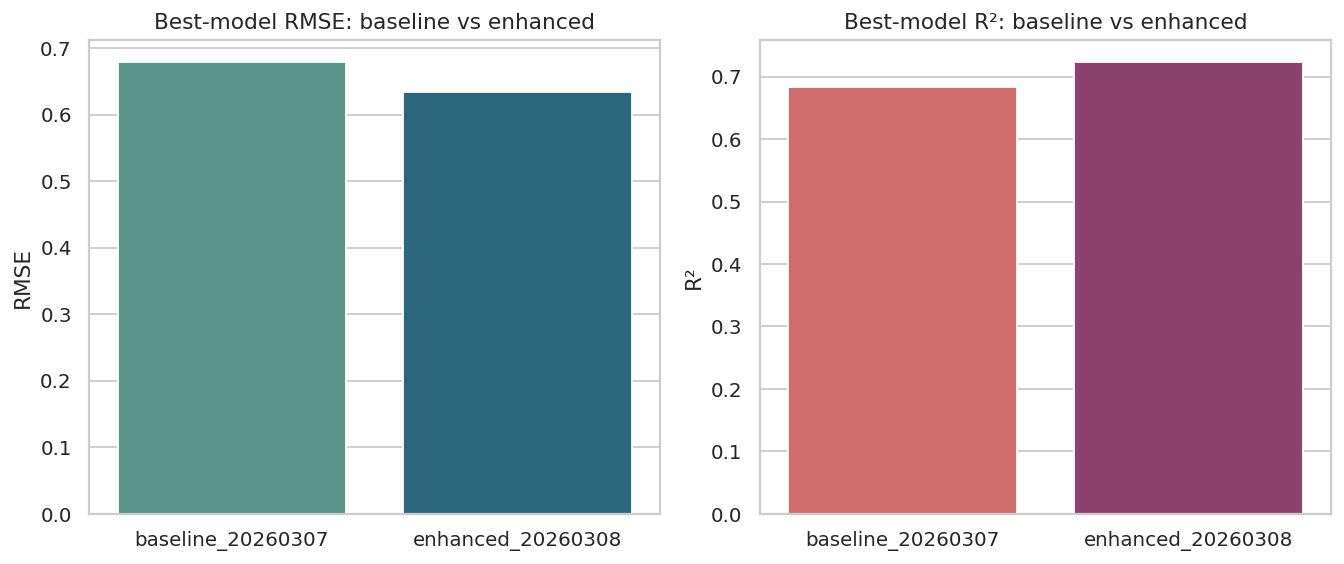
\includegraphics{../figures/14_baseline_vs_enhanced.png}

\hypertarget{ux56fe2ux4e25ux683c-scaffold-ux9a8cux8bc1ux7ed3ux679c}{%
\subsubsection{图2：严格 scaffold
验证结果}\label{ux56fe2ux4e25ux683c-scaffold-ux9a8cux8bc1ux7ed3ux679c}}

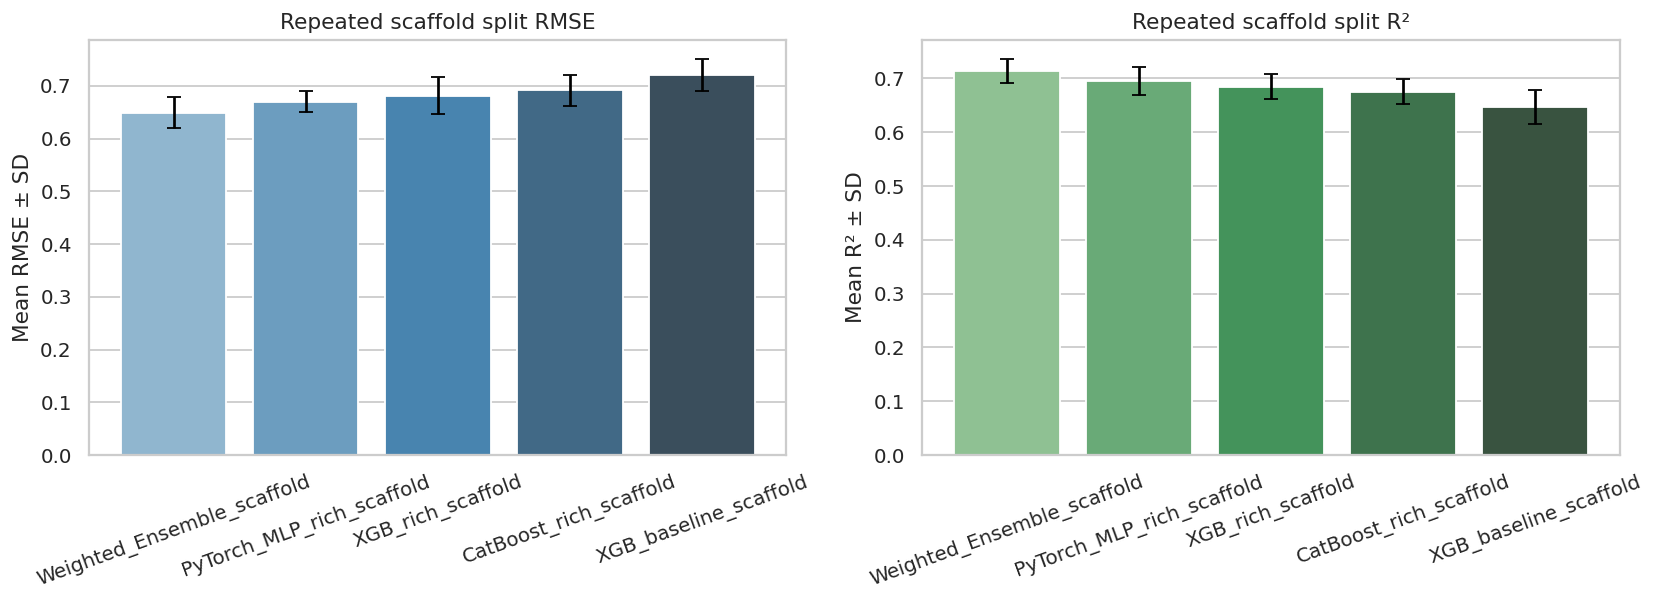
\includegraphics{../figures/16_scaffold_repeat_summary.png}

\hypertarget{ux56fe3shap-ux5168ux5c40ux91cdux8981ux7279ux5f81}{%
\subsubsection{图3：SHAP
全局重要特征}\label{ux56fe3shap-ux5168ux5c40ux91cdux8981ux7279ux5f81}}

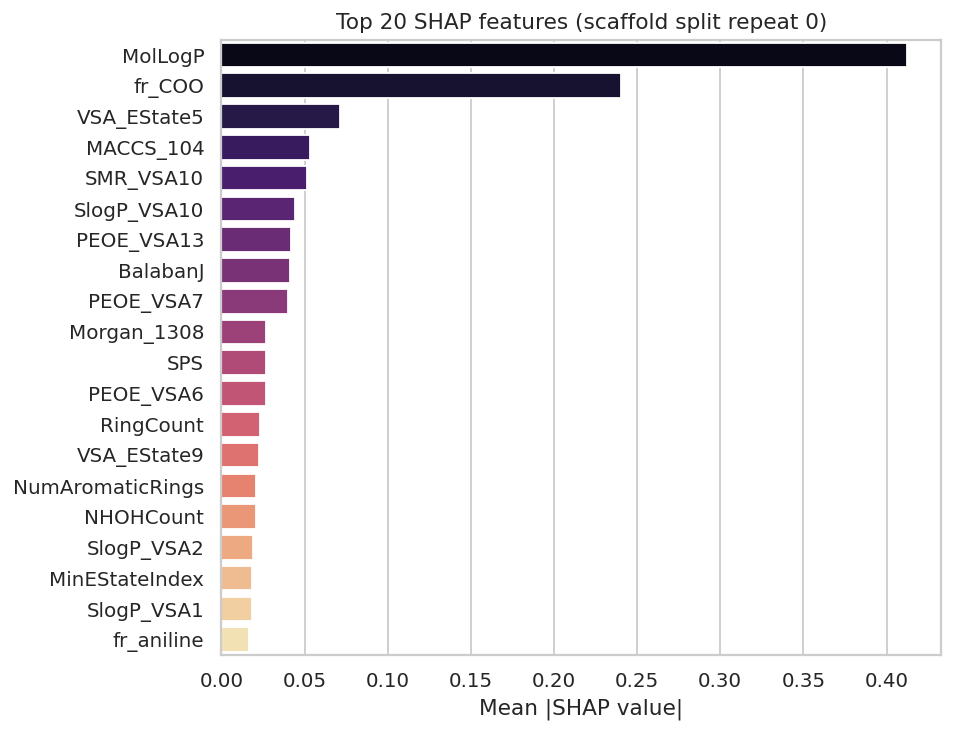
\includegraphics{../figures/19_shap_top20_bar.png}

\hypertarget{ux56fe4ux5c40ux90e8ux89e3ux91caux4ee3ux8868ux5206ux5b50}{%
\subsubsection{图4：局部解释代表分子}\label{ux56fe4ux5c40ux90e8ux89e3ux91caux4ee3ux8868ux5206ux5b50}}

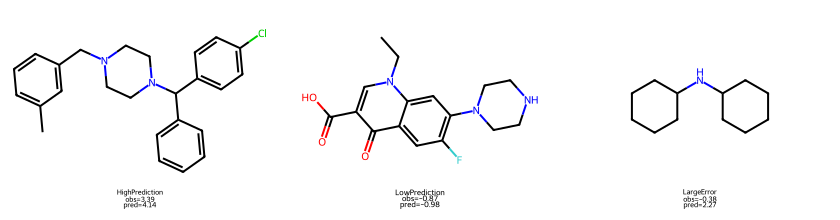
\includegraphics{../figures/22_shap_case_molecules.png}

\begin{center}\rule{0.5\linewidth}{0.5pt}\end{center}

\hypertarget{ux9644ux5f55-cux5efaux8baeux8001ux5e08ux8ffdux95eeux65f6ux7684ux6807ux51c6ux56deux7b54ux6a21ux677f}{%
\subsection{附录
C：建议老师追问时的标准回答模板}\label{ux9644ux5f55-cux5efaux8baeux8001ux5e08ux8ffdux95eeux65f6ux7684ux6807ux51c6ux56deux7b54ux6a21ux677f}}

\hypertarget{ux95eeux8fd9ux4e2aux9879ux76eeux6700ux91cdux8981ux7684ux521bux65b0ux70b9ux662fux4ec0ux4e48}{%
\subsubsection{问：这个项目最重要的创新点是什么？}\label{ux95eeux8fd9ux4e2aux9879ux76eeux6700ux91cdux8981ux7684ux521bux65b0ux70b9ux662fux4ec0ux4e48}}

答：不是单纯追求一个更高的分数，而是把真实公开数据、结构增强建模、严格验证、SHAP
解释和在线平台结合起来，使它既有科研严谨性，也有展示和应用价值。

\hypertarget{ux95eeux4e3aux4ec0ux4e48ux4f60ux8bf4ux5b83ux53efux89e3ux91ca}{%
\subsubsection{问：为什么你说它``可解释''？}\label{ux95eeux4e3aux4ec0ux4e48ux4f60ux8bf4ux5b83ux53efux89e3ux91ca}}

答：因为不仅有全局重要特征，还有对单个分子的局部 SHAP
解释，可以知道哪些特征在把预测往上推、哪些在往下拉。

\hypertarget{ux95eegemini-ux5728ux8fd9ux91ccux662fux4e0dux662fux66ffux4ee3ux5206ux6790}{%
\subsubsection{问：Gemini
在这里是不是``替代分析''？}\label{ux95eegemini-ux5728ux8fd9ux91ccux662fux4e0dux662fux66ffux4ee3ux5206ux6790}}

答：不是。Gemini
不负责做核心预测，只负责把已经得到的模型结果翻译成更自然的药学和项目说明，所以它是解释层，不是核心科学结论来源。

\hypertarget{ux95eeux4e3aux4ec0ux4e48ux5e73ux53f0ux5316ux4e5fux91cdux8981}{%
\subsubsection{问：为什么平台化也重要？}\label{ux95eeux4e3aux4ec0ux4e48ux5e73ux53f0ux5316ux4e5fux91cdux8981}}

答：因为平台化说明这个项目不是停留在离线脚本层面，而是已经具备``别人可以直接访问和调用''的工具属性，这对计算机和交叉项目尤其重要。

\end{document}
